\RequirePackage[l2tabu, orthodox]{nag}
\documentclass[12pt]{article}
\usepackage[T1]{fontenc}
\usepackage[utf8]{inputenc}
\usepackage[french]{babel}
\usepackage{amsthm,amssymb,amsmath,xcolor}
\usepackage{setspace}
\doublespacing
\usepackage{geometry}
\geometry{
    a4paper,
    total={170mm,257mm},
}
\usepackage{graphicx}
\graphicspath{ {./} }
\usepackage{microtype}
\usepackage{todonotes}
\usepackage{hyperref}
\hypersetup{
    colorlinks=true,
    linkcolor=blue,
    filecolor=magenta,
    urlcolor=cyan,
}

\author{Efe ERKEN}
\date{\today}
\title{Rapport Projet ``Liste de tâches''}

\begin{document}
\maketitle

\section{Modèle E/A}
\begin{center}
	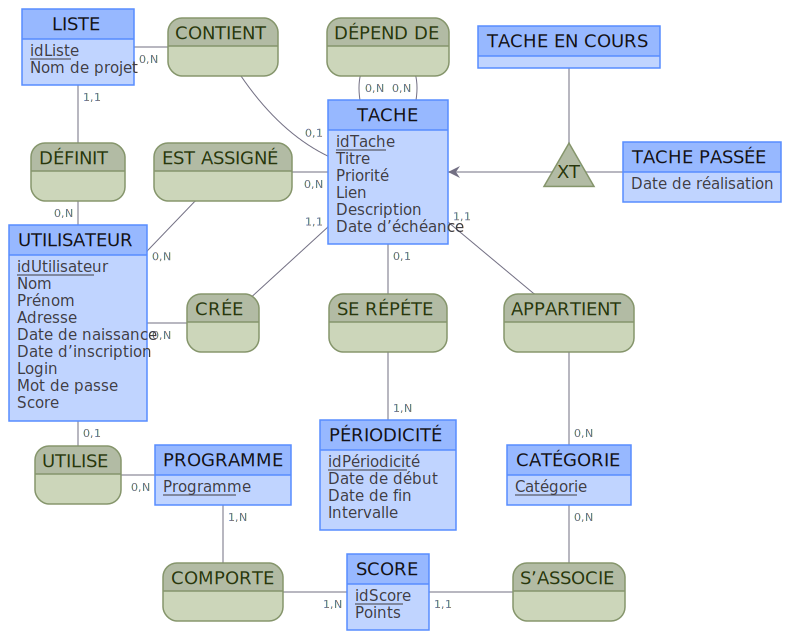
\includegraphics[scale=0.8]{modeleEA.png}
\end{center}

\section{Modèle relationnel}
\input{mld.tex}

\section{Choix d'implémentation}
Tout d'abord, petit avertissement. J'ai fait le choix d'utiliser
\href{https://dbeaver.io/}{\texttt{DBeaver}} comme client SQL et environnement
de dévéloppement pour la première partie du projet. J'ai testé et assuré
fonctionnel mon travail à l'aide de cet outil. Mais pendant la deuxième partie
où je travaillais sur des blocs PL/SQL, j'ai découvert que \texttt{DBeaver} ne
marchait pas très bien avec ces blocs.  Puisque mon projet était adapté pour
\texttt{DBeaver} des erreurs se manifestait à l'execution avec d'autres outils
comme \texttt{SQLplus}, \texttt{SQL Developer} ou même \texttt{JetBrains
DataGrip}. Je n'ai pas conduit de tests avec ces outils mais je sais que
certaines formes de syntaxe \texttt{DBeaver} ne marche pas sur \texttt{SQLplus}
et vice-versa. (Notamment il ne se trouvait pas le charactère ``\texttt{/}''
dans mes scripts qui est nécessaire avec \texttt{SQLplus}.) J'ai donc fait la
décision d'adapter mes scripts à \texttt{SQLplus} en incluant le charactère
``\texttt{/}'' aux bons endroits et aussi en fournissant désormais un autre
script \texttt{main} dédié à \texttt{SQLplus}. Tout est donc assuré en bon état
de marche avec \texttt{SQLplus}.  Si vous voulez utiliser \texttt{DBeaver} et
son script à lui il faut veiller à supprimer les charactères ``\texttt{/}'' à la
fin des blocs PL/SQL dans un premier temps.  Et dans un deuxième temps mettre en
commentaire les blocs PL/SQL de création de fonction et de procédure pour après
les séléctionner en bloc et les executer manuellement. Sinon DBeaver sépare ces
blocs en petits morceaux et des erreurs surviennent coté BDD disant ``expression
invalide''.  DBeaver ne parse pas bien ce genre de blocs PL/SQL tout simplement
lors de l'execution en mode fichier complet. \\

Ensuite, j'ai respecté les détails du sujet dans la limite de ma compréhension
de ce dernier. J'ai repris la correction proposée pour corriger ma version du
projet. Je ne me suis pas basé entièrment sur la correction mais je l'ai adapté
pour mes besoins comme je l'ai compris. Dans mon implémentation, il y a bien
deux tables pour les tâches actuelles et les tâches passées. Pour s'assurer que
sur l'ensemble des deux tables tâche, les identifiants soient unique et que les
tables qui ont comme clé étrangère des tâches, réfèrent bien à des tâches
existantes, j'ai crée une table en plus (la super table) pour rien d'autre que
de contenir les identifiants des tâches globalement. Des déclencheurs vont
assurer l'unicité des identifiants lors des insertions et des mises à jour ainsi
que de servir à effacer en cascade les n-uplets qui réfèrent à des tâches qui
viennent d'être supprimées. D'autres contraintes qui nécessitent de lire des
tables ou des comparaisons avec la date actuelle vont aussi devoir être
implémentées dynamiquement. \\

Une liste et un projet sont vus comme la même entité. Au lieu d'avoir une autre
table projet, j'ai integré un attribut ``nom de projet'' dans la table liste.
Une liste est un projet, un projet est une liste. C'est une manière d'organiser
ses tâches tout simplement. \\

Les listes vides (avec aucune tâche comme contenu) sont autorisées. Les tâches
peuvent être dans aucune liste. Toute tâche appartient à un utilisateur qui est
son créateur logiquement parlant, cela est stocké en tant qu'attribut dans une
tâche. Les utilisateurs ne peuvent pas être assignés à leurs propres tâches.
Une tâche ne peut pas dépendre d'elle même, non plus d'intérdependence entre des
tâches (cycles). \\

Le score (le nombre de points) est stocké en tant qu'attribut dans la table
utilisateur pour adhérer à l'indication du déclancheur 1 dans le sujet.  Les
programmes sont nommées et sont utilisés par des utilisateur optionnellement.
Ils comporte au moins un score et chaque score est associé à une catégorie de
tâche. Ainsi on peut dire que les utilisateurs gagnent ou perdent le nombre de
points indiqué dans le score pour les tâches correspondants par leurs catégories
en fonction de si elles sont bien accomplies ou dépassées.  Le programme est un
attribut de la table utilisateur. \\

La périodicité existe maintenant dans sa table à part mais plusieurs tâches
peuvent réferer à une même entrée de périodicité. Cela sert à identifier
plusieurs instances d'une tâche périodique si on veut supprimer une telle tâche
en un coup avec toutes ses instances qui sont par exemple créées par le
déclancheur numéro 2 du sujet. Cela aide aussi à identifier une suite de tâches
périodiques comme les instances d'une seule tâche qui est en fait périodique.
Comme cela on peut aussi éviter de compter ces multiples instances comme des
tâches à part dans le compte global des tâches. \\

Je n'ai pas eu assez de temps pour implémenter les déclancheurs que j'ai décrit
comme contrainte d'intégrité en version texte (identifié par \texttt{PLxx}), non
plus les deux déclancheurs demandés dans le sujet même s'ils avaient l'air pas
trop difficile. À part cela, j'ai fait toutes les autres demandes du sujet telle
que les requêtes, les procédures, les fonctions et d'autres. La troisième
fonction était très compliquée. Je l'ai tenté quand même mais ça n'adhère pas
vraiment à la demande du sujet avec un mécanisme de comparaison de mots valides.

\input{contraintes.tex}


\end{document}

